\chapter{Features}

\section{Kompatibilität}

Die Vorlage funktioniert mit pdf\LaTeX, \XeLaTeX und \LuaLaTeX. Das mitgelieferte \texttt{Makefile}
ruft \XeLaTeX auf.

Die Vorlage ist bereits eingerichtet, um die Verwendung von deutschen Sonderzeichen und
einigen Unicode-Symbolen (z.B. π) zu ermöglichen. Das klappt gut mit \XeTeX und den
\texttt{CMU}-Schriften, sonst eher sporadisch.

Das \texttt{Makefile} wurde nur auf GNU/Linux-Systemen getestet. Es funktioniert wahrscheinlich
auf anderen unixoiden Betriebssystemen, aber eher nicht auf Windows.

\section{Latexrun}

Diese Vorlage benützt \texttt{latexrun}\cite{latexrun}.
Latexrun ruft \LaTeX genau so oft auf wie nötig,
um alle Änderungen der Eingabedateien in die Ausgabedatei zu übernehmen.
Außerdem versucht latexrun, Fehlermeldungen und Warnungen
der richtigen Quelltextdatei und Quelltextzeile zuzuordnen.
Das klappt in den allermeisten Fällen, aber nicht immer. Manchmal kann \texttt{latexrun}
keine Zeilennummer finden, dann muss man den Fehler von Hand suchen.

Das Programm \texttt{latexrun} ist mitgeliefert. Das \texttt{Makefile} ruft \texttt{latexrun}
für alle \texttt{.tex}-Dateien im obersten Verzeichnis auf. Ausgabeformat ist immer PDF.

\section{Dot-Grafiken}

Das Makefile enthält eine Regel zur Konvertierung von Graphen im \texttt{dot}-Format mittels
der GraphViz-Programmsuite \cite{gansner2000open}.

Die Abbildung \ref{fig:dotgraph} zeigt einen sehr einfachen gerichteten Graphen,
der als PDF konvertiert eingebunden ist.

\begin{figure}[!ht]
    \centering
    \caption{Beispielgraph}
    \label{fig:dotgraph}
    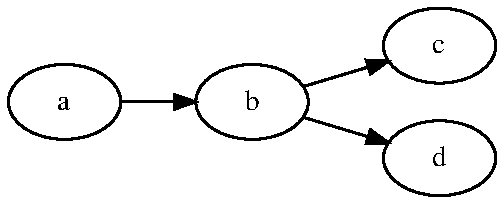
\includegraphics[width=0.8\textwidth]{img/examplegraph}
    \source{Eigene Darstellung}
\end{figure}

\section{SVG-Konvertierung}

Auch integriert ist eine Regel, die SVG-Dateien in von pdf\LaTeX verwendbare PDF-Dokumente konvertiert. Zur Konvertierung wird Inkscape\cite{inkscape} als Kommandozeilenprogramm aufgerufen.
Ein Beispiel-SVG ist in Abbildung \ref{fig:cartman} gezeigt.

\begin{figure}[!ht]
    \centering
    \caption{Beispiel-SVG: Cartman}
    \label{fig:cartman}
    
\includegraphics[width=0.3\textwidth]{img/cartman}
    \source{\url{https://dev.w3.org/SVG/tools/svgweb/samples/svg-files/cartman.svg}}
\end{figure}
